\begin{frame}{Introduction : Les classiques de ctf}
    \large{\centerline{\textbf{Cinq challenges de démarrage}}}

\end{frame}

%------------------------------------------------
%------------------------------------------------

\begin{frame}{RSA-WTF \FiveStar (speedrun)\hfill 202 résolutions}
    \begin{columns}[c]
        \column{.45\textwidth}
        \begin{center}                  
            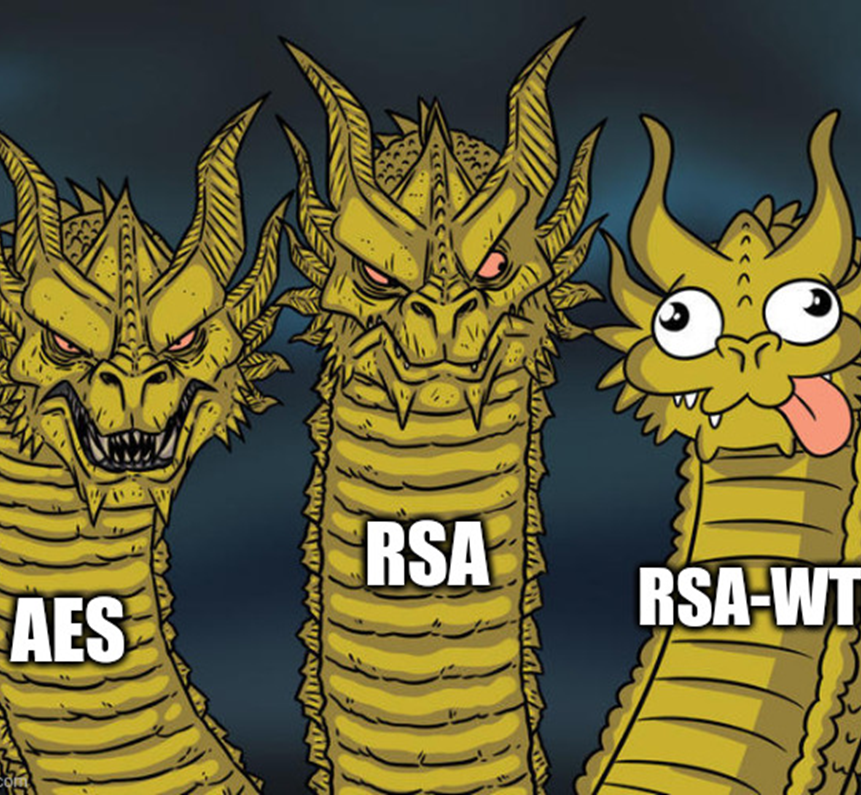
\includegraphics[width=0.8\textwidth]{img/meme/rsa-wtf-intro.png}
        \end{center}

        \column{.65\textwidth} % 
           \begin{outline}
               \1 Objectif
                \2 Récupérer \u{$d$} aléatoire sur 666 bits

            \pause
               \1 Données
                \2 $\k{d_p} = \u{d}^{-1} \mod (\k{p}-1)$
                \2 $\k{d_q} = \u{d}^{-1} \mod (\k{q}-1)$

                \pause
                
                \2 $\k{p, q}$ sur 512 bits

            \pause
               \1 Solution
                \2 Théorème des restes chinois pour avoir
                    \[d \mod lcm(p-1,q-1) \]
            
            \pause
               \1 First Blood en 65 secondes \flag{}
           \end{outline}
    \end{columns}
\end{frame}

%------------------------------------------------
%------------------------------------------------

\begin{frame}{CocoRiCo \FiveStar \hfill 366 résolutions}
    \begin{columns}[c]
        \column{.45\textwidth}
        \begin{center}                  
            
\includegraphics[width=0.8\textwidth]{img/meme/cocorico.png}
        \end{center}

        \column{.65\textwidth} % 
           \begin{outline}
               \1 Objectif
                \2 Forger un chiffrement + authentification
               \1 Données
                \2 Accès à un oracle
               \1 Solution
                \2 Malléabilité d'AES-CTR / AES-OFB
               \1 First Blood en 7 minutes \flag{}
           \end{outline}
    \end{columns}
\end{frame}

%------------------------------------------------
%------------------------------------------------

\begin{frame}{Problèmeuh \FiveStar \FiveStar \hfill 156 résolutions}
    \begin{columns}[c]
        \column{.45\textwidth}
        \begin{center}                  
            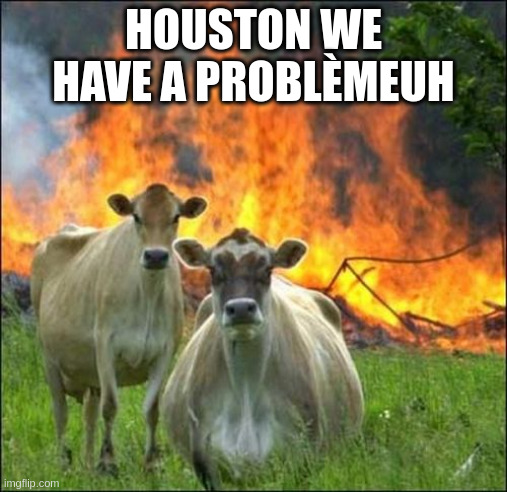
\includegraphics[width=0.8\textwidth]{img/meme/problemeuh-intro.png}
        \end{center}

        \column{.65\textwidth} % 
           \begin{outline}
               \1 Objectif
                \2 Résoudre un système d'équation diophantienne
                \[\left\{
                    \begin{array}{r c l}
                        \u{a} &=&  487 \u{c} \\
                        59\u{a} &=& 485 \u{b} \\
                        \u{x} ^ 2 &=& \u{a} + \u{b} \\
                        \u{y} (3 \u{y} - 1) &=& 2 \u{b} \\
                    \end{array}
                \right.\]
               \1 Solution
                \2 Se ramener à l'équation de Pell :
                 \[(6\u{y} - 1)^2 - 145710941544 \u{k}^2 = 1\]
               \1 Peut se résoudre avec des fractions continues
               \1 \url{https://www.alpertron.com.ar/METHODS.HTM} \flag{}
           \end{outline}
    \end{columns}
\end{frame}

%------------------------------------------------
%------------------------------------------------

\begin{frame}{La quête de l'anneau \FiveStar \hfill 585 résolutions}
    \begin{columns}[c]
        \column{.45\textwidth}
        \begin{center}                  
            
\includegraphics[width=0.8\textwidth]{img/meme/la-quete-intro.png}
        \end{center}

        \column{.65\textwidth} % 
           \begin{outline}
               \1 Objectif
                \2 Résoudre des équations modulo $\u{s}$ aléatoire 
                \2 $E : \u{m} \mapsto \k{IV}\cdot \u{m} \mod \u{s} = \k{c}$
                \2 $E^{-1} : \k{c} \mapsto \u{IV^{-1}}\cdot \k{c} \mod \u{s} = \u{m}$

                \vspace{0.3cm}
                \pause
                
               \1 Données
                \2 Deux clairs connu $E(\k{m_1}) = \k{c_1}$ et $E(\k{m_2}) = \k{c_2}$
                \2 Un message à déchiffrer $\u{m_3}$ sachant $\k{c_3}$
               
                \vspace{0.3cm}
                \pause 
                
               \1 Solution
                \2 $\left\{ \begin{array}{r c l} \k{c_1} &=& \k{IV_1}\cdot\k{m_1}+\u{k_1}\u{s} \\
                        \k{c_2} &=& \k{IV_2}\cdot\k{m_2} +\u{k_2}\u{s} \\
                    \end{array}
                \right.$

                
                \pause
                \2 $s = PGCD(\k{c_1}-\k{IV_1}\cdot\k{m_1},\k{c_2}-\k{IV_2}\cdot\k{m_2})$ \flag{}
           \end{outline}
    \end{columns}
\end{frame}


%------------------------------------------------
%------------------------------------------------

\begin{frame}{La revanche de Sauron \FiveStar \FiveStar (speedrun) \hfill 9 résolutions}
    \begin{columns}[c]
        \column{.45\textwidth}
        \begin{center}                  
            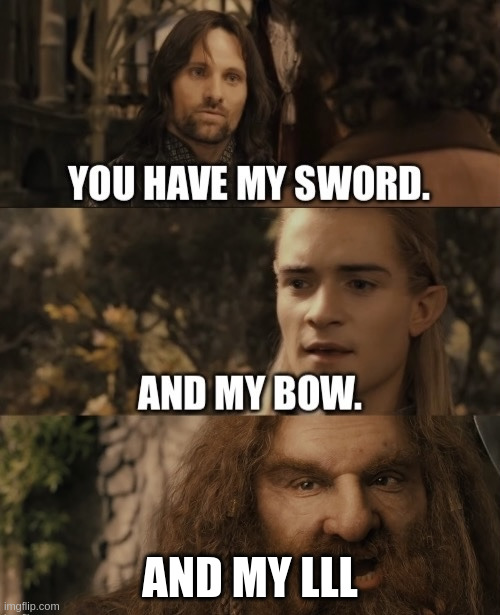
\includegraphics[width=0.8\textwidth]{img/meme/la-revanche-intro.png}
        \end{center}

        \column{.65\textwidth} % 
           \begin{outline}
            \1 Objectif
                \2 Résoudre des équations modulo $\u{s}$ aléatoire 
                \2 $E : \u{m} \mapsto \k{IV}\cdot \u{m} \mod \u{s} = \k{c}$
                \2 $E^{-1} : \k{c} \mapsto \u{IV^{-1}}\cdot \k{c} \mod \u{s} = \u{m}$

               \1 Données
                \2 Les chiffrés : $E(\u{m_1})=\k{c_1}$ et $E(\u{m_2}) = \k{c_2}$

                \pause
                
               \1 Solution
                \2  $\left\{ \begin{array}{r c l} \k{c_1} &=& \k{IV_1}\cdot\u{m_1}+\u{k_1}\u{s} \\
                        \k{c_2} &=& \k{IV_2}\cdot\u{m_2} +\u{k_2}\u{s} \\
                    \end{array}
                \right.$
                
                \vspace{0.3cm}
                
                \2 $\k{c_1}\u{k_2} - \k{IV_1}\u{m_1}\u{k_2} - \k{c_2}\u{k_1} +  \k{IV_2}\u{m_2}\u{k_1} =  0$

                \pause
                \vspace{0.3cm}

                \pause 
                
                \2 $\u{s}$ et $\k{IV_i}$ font 1024 bits, $\u{m_i}$ font $256$ bits
            \1 Résoudre avec Coppersmith ou LLL ?
           \end{outline}
    \end{columns}
\end{frame}

%------------------------------------------------
%------------------------------------------------

\begin{frame}{Coppersmith / LLL}
\begin{block}{Utilisation de l'algorithme LLL en ctf}
    Trouve des combinaisons linéaires anormalement petites de vecteurs.
\end{block}

\pause

\vspace{-0.4cm}

     \[
        \begin{tikzpicture}[baseline=(eq.base)]
            \node (eq) at (0,0) {$\k{c_1}\u{k_2} - \k{IV_1}\u{m_1}\u{k_2} - \k{c_2}\u{k_1} +  \k{IV_2}\u{m_2}\u{k_1} =  0$};

            \foreach \x/\label in {
                -2.8/1024,
                -1.55/1024,
                 0./1024,
                 1.2/1024 bits
            } {
                \draw[<-, thick] (\x,0.2) -- ++(0,0.6) node[above] {\scriptsize \label};
            }
        \end{tikzpicture}
    \]

\pause

\begin{outline}
    \1 $0$ est engendré par $(\k{c_1})$, $(\k{IV_1})$, $(\k{c_2})$, $(\k{IV_2})$ 
        \pause
        \2[$\longrightarrow$]  LLL retourne bien $0$
    \1 Comment retrouver les coefficients utilisés?
    \pause
    \1 $\left[
    \begin{array}{ r c c c c}
        \k{c_1},  &1, &0, &0, &0  \\
        -\k{IV_1},&0, &1, &0, &0 \\
        -\k{c_2}, &0, &0, &1, &0 \\
        \k{IV_2}, &0, &0, &0, &1 \\
    \end{array}
    \right]$ engendre le vecteur $(0, \u{k_2},\u{m_1}\u{k_2},\u{k_1},\u{m_2}\u{k_1})$
    \pause
    \1 Il a pour taille (1, 256, 512, 256,512) bits. Est-il anormalement petit?
    \pause 
     \2[$\longrightarrow$] LLL trouve un vecteur de $(254, 251, 256, 255, 257)$ bits
\end{outline}
\end{frame} 

%------------------------------------------------
%------------------------------------------------



\begin{frame}{Changer la géométrie d'un réseau}

\begin{outline}
    \1 $\left[
    \begin{array}{r c c c c}
        \k{c_1} \times \mathbf{B},  &1, &0, &0, &0  \\
        -\k{IV_1} \times \mathbf{B}, &0, &1, &0, &0 \\
        -\k{c_2} \times \mathbf{B}, &0, &0, &1, &0 \\
        \k{IV_2} \times \mathbf{B}, &0, &0, &0, &1 \\
    \end{array}
    \right]$ engendre toujours $(0, \u{k_2},\u{m_1}\u{k_2},\u{k_1},\u{m_2}\u{k_1})$
    
    \pause \1 Un B gigantesque forcera la première composante à 0
        \2[$\longrightarrow$] LLL trouve un vecteur de taille $(1, 339, 339, 340, 341)$ bits
    \pause
    
    \vspace{0.5cm}
    
     \1 $\left[
    \begin{array}{r c c c c}
        \k{c_1} \times \mathbf{B},  &\mathbf{2^{256}}, &0, &0, &0  \\
        -\k{IV_1} \times \mathbf{B}, &0, &1, &0, &0 \\
        -\k{c_2} \times \mathbf{B}, &0, &0, &\mathbf{2^{256}}, &0 \\
        \k{IV_2} \times \mathbf{B}, &0, &0, &0, &1 \\
    \end{array}
    \right]$ engendre $(0, 2^{256}\u{k_2},\u{m_1}\u{k_2},2^{256}\u{k_1},\u{m_2}\u{k_1})$

        \pause
        
    \2[$\longrightarrow$] C'est bien le vecteur trouvé par LLL \flag{}
\end{outline}
\end{frame} 


